% Options for packages loaded elsewhere
\PassOptionsToPackage{unicode}{hyperref}
\PassOptionsToPackage{hyphens}{url}
\PassOptionsToPackage{dvipsnames,svgnames,x11names}{xcolor}
%
\documentclass[
  a4paper,
]{article}

\usepackage{amsmath,amssymb}
\usepackage{iftex}
\ifPDFTeX
  \usepackage[T1]{fontenc}
  \usepackage[utf8]{inputenc}
  \usepackage{textcomp} % provide euro and other symbols
\else % if luatex or xetex
  \usepackage{unicode-math}
  \defaultfontfeatures{Scale=MatchLowercase}
  \defaultfontfeatures[\rmfamily]{Ligatures=TeX,Scale=1}
\fi
\usepackage{lmodern}
\ifPDFTeX\else  
    % xetex/luatex font selection
\fi
% Use upquote if available, for straight quotes in verbatim environments
\IfFileExists{upquote.sty}{\usepackage{upquote}}{}
\IfFileExists{microtype.sty}{% use microtype if available
  \usepackage[]{microtype}
  \UseMicrotypeSet[protrusion]{basicmath} % disable protrusion for tt fonts
}{}
\makeatletter
\@ifundefined{KOMAClassName}{% if non-KOMA class
  \IfFileExists{parskip.sty}{%
    \usepackage{parskip}
  }{% else
    \setlength{\parindent}{0pt}
    \setlength{\parskip}{6pt plus 2pt minus 1pt}}
}{% if KOMA class
  \KOMAoptions{parskip=half}}
\makeatother
\usepackage{xcolor}
\usepackage[top=2.54cm,right=2.54cm,bottom=2.54cm,left=2.54cm]{geometry}
\setlength{\emergencystretch}{3em} % prevent overfull lines
\setcounter{secnumdepth}{-\maxdimen} % remove section numbering
% Make \paragraph and \subparagraph free-standing
\ifx\paragraph\undefined\else
  \let\oldparagraph\paragraph
  \renewcommand{\paragraph}[1]{\oldparagraph{#1}\mbox{}}
\fi
\ifx\subparagraph\undefined\else
  \let\oldsubparagraph\subparagraph
  \renewcommand{\subparagraph}[1]{\oldsubparagraph{#1}\mbox{}}
\fi

\usepackage{color}
\usepackage{fancyvrb}
\newcommand{\VerbBar}{|}
\newcommand{\VERB}{\Verb[commandchars=\\\{\}]}
\DefineVerbatimEnvironment{Highlighting}{Verbatim}{commandchars=\\\{\}}
% Add ',fontsize=\small' for more characters per line
\newenvironment{Shaded}{}{}
\newcommand{\AlertTok}[1]{\textcolor[rgb]{1.00,0.33,0.33}{\textbf{#1}}}
\newcommand{\AnnotationTok}[1]{\textcolor[rgb]{0.42,0.45,0.49}{#1}}
\newcommand{\AttributeTok}[1]{\textcolor[rgb]{0.84,0.23,0.29}{#1}}
\newcommand{\BaseNTok}[1]{\textcolor[rgb]{0.00,0.36,0.77}{#1}}
\newcommand{\BuiltInTok}[1]{\textcolor[rgb]{0.84,0.23,0.29}{#1}}
\newcommand{\CharTok}[1]{\textcolor[rgb]{0.01,0.18,0.38}{#1}}
\newcommand{\CommentTok}[1]{\textcolor[rgb]{0.42,0.45,0.49}{#1}}
\newcommand{\CommentVarTok}[1]{\textcolor[rgb]{0.42,0.45,0.49}{#1}}
\newcommand{\ConstantTok}[1]{\textcolor[rgb]{0.00,0.36,0.77}{#1}}
\newcommand{\ControlFlowTok}[1]{\textcolor[rgb]{0.84,0.23,0.29}{#1}}
\newcommand{\DataTypeTok}[1]{\textcolor[rgb]{0.84,0.23,0.29}{#1}}
\newcommand{\DecValTok}[1]{\textcolor[rgb]{0.00,0.36,0.77}{#1}}
\newcommand{\DocumentationTok}[1]{\textcolor[rgb]{0.42,0.45,0.49}{#1}}
\newcommand{\ErrorTok}[1]{\textcolor[rgb]{1.00,0.33,0.33}{\underline{#1}}}
\newcommand{\ExtensionTok}[1]{\textcolor[rgb]{0.84,0.23,0.29}{\textbf{#1}}}
\newcommand{\FloatTok}[1]{\textcolor[rgb]{0.00,0.36,0.77}{#1}}
\newcommand{\FunctionTok}[1]{\textcolor[rgb]{0.44,0.26,0.76}{#1}}
\newcommand{\ImportTok}[1]{\textcolor[rgb]{0.01,0.18,0.38}{#1}}
\newcommand{\InformationTok}[1]{\textcolor[rgb]{0.42,0.45,0.49}{#1}}
\newcommand{\KeywordTok}[1]{\textcolor[rgb]{0.84,0.23,0.29}{#1}}
\newcommand{\NormalTok}[1]{\textcolor[rgb]{0.14,0.16,0.18}{#1}}
\newcommand{\OperatorTok}[1]{\textcolor[rgb]{0.14,0.16,0.18}{#1}}
\newcommand{\OtherTok}[1]{\textcolor[rgb]{0.44,0.26,0.76}{#1}}
\newcommand{\PreprocessorTok}[1]{\textcolor[rgb]{0.84,0.23,0.29}{#1}}
\newcommand{\RegionMarkerTok}[1]{\textcolor[rgb]{0.42,0.45,0.49}{#1}}
\newcommand{\SpecialCharTok}[1]{\textcolor[rgb]{0.00,0.36,0.77}{#1}}
\newcommand{\SpecialStringTok}[1]{\textcolor[rgb]{0.01,0.18,0.38}{#1}}
\newcommand{\StringTok}[1]{\textcolor[rgb]{0.01,0.18,0.38}{#1}}
\newcommand{\VariableTok}[1]{\textcolor[rgb]{0.89,0.38,0.04}{#1}}
\newcommand{\VerbatimStringTok}[1]{\textcolor[rgb]{0.01,0.18,0.38}{#1}}
\newcommand{\WarningTok}[1]{\textcolor[rgb]{1.00,0.33,0.33}{#1}}

\providecommand{\tightlist}{%
  \setlength{\itemsep}{0pt}\setlength{\parskip}{0pt}}\usepackage{longtable,booktabs,array}
\usepackage{calc} % for calculating minipage widths
% Correct order of tables after \paragraph or \subparagraph
\usepackage{etoolbox}
\makeatletter
\patchcmd\longtable{\par}{\if@noskipsec\mbox{}\fi\par}{}{}
\makeatother
% Allow footnotes in longtable head/foot
\IfFileExists{footnotehyper.sty}{\usepackage{footnotehyper}}{\usepackage{footnote}}
\makesavenoteenv{longtable}
\usepackage{graphicx}
\makeatletter
\def\maxwidth{\ifdim\Gin@nat@width>\linewidth\linewidth\else\Gin@nat@width\fi}
\def\maxheight{\ifdim\Gin@nat@height>\textheight\textheight\else\Gin@nat@height\fi}
\makeatother
% Scale images if necessary, so that they will not overflow the page
% margins by default, and it is still possible to overwrite the defaults
% using explicit options in \includegraphics[width, height, ...]{}
\setkeys{Gin}{width=\maxwidth,height=\maxheight,keepaspectratio}
% Set default figure placement to htbp
\makeatletter
\def\fps@figure{htbp}
\makeatother

\makeatletter
\makeatother
\makeatletter
\makeatother
\makeatletter
\@ifpackageloaded{caption}{}{\usepackage{caption}}
\AtBeginDocument{%
\ifdefined\contentsname
  \renewcommand*\contentsname{Tabla de contenidos}
\else
  \newcommand\contentsname{Tabla de contenidos}
\fi
\ifdefined\listfigurename
  \renewcommand*\listfigurename{Listado de Figuras}
\else
  \newcommand\listfigurename{Listado de Figuras}
\fi
\ifdefined\listtablename
  \renewcommand*\listtablename{Listado de Tablas}
\else
  \newcommand\listtablename{Listado de Tablas}
\fi
\ifdefined\figurename
  \renewcommand*\figurename{Figura}
\else
  \newcommand\figurename{Figura}
\fi
\ifdefined\tablename
  \renewcommand*\tablename{Tabla}
\else
  \newcommand\tablename{Tabla}
\fi
}
\@ifpackageloaded{float}{}{\usepackage{float}}
\floatstyle{ruled}
\@ifundefined{c@chapter}{\newfloat{codelisting}{h}{lop}}{\newfloat{codelisting}{h}{lop}[chapter]}
\floatname{codelisting}{Listado}
\newcommand*\listoflistings{\listof{codelisting}{Listado de Listados}}
\makeatother
\makeatletter
\@ifpackageloaded{caption}{}{\usepackage{caption}}
\@ifpackageloaded{subcaption}{}{\usepackage{subcaption}}
\makeatother
\makeatletter
\@ifpackageloaded{tcolorbox}{}{\usepackage[skins,breakable]{tcolorbox}}
\makeatother
\makeatletter
\@ifundefined{shadecolor}{\definecolor{shadecolor}{rgb}{.97, .97, .97}}
\makeatother
\makeatletter
\makeatother
\makeatletter
\makeatother
\ifLuaTeX
\usepackage[bidi=basic]{babel}
\else
\usepackage[bidi=default]{babel}
\fi
\babelprovide[main,import]{spanish}
% get rid of language-specific shorthands (see #6817):
\let\LanguageShortHands\languageshorthands
\def\languageshorthands#1{}
\ifLuaTeX
  \usepackage{selnolig}  % disable illegal ligatures
\fi
\usepackage[]{biblatex}
\addbibresource{../../../../references.bib}
\IfFileExists{bookmark.sty}{\usepackage{bookmark}}{\usepackage{hyperref}}
\IfFileExists{xurl.sty}{\usepackage{xurl}}{} % add URL line breaks if available
\urlstyle{same} % disable monospaced font for URLs
\hypersetup{
  pdftitle={Gráficos avanzados con python},
  pdfauthor={Edison Achalma},
  pdflang={es},
  colorlinks=true,
  linkcolor={blue},
  filecolor={Maroon},
  citecolor={Blue},
  urlcolor={Blue},
  pdfcreator={LaTeX via pandoc}}

\title{Gráficos avanzados con python}
\usepackage{etoolbox}
\makeatletter
\providecommand{\subtitle}[1]{% add subtitle to \maketitle
  \apptocmd{\@title}{\par {\large #1 \par}}{}{}
}
\makeatother
\subtitle{Sumérgete en técnicas avanzadas de visualización, desde
gráficos 3D hasta interactivos y mapas temáticos}
\author{Edison Achalma}
\date{2023-06-30}

\begin{document}
\maketitle
\ifdefined\Shaded\renewenvironment{Shaded}{\begin{tcolorbox}[interior hidden, frame hidden, borderline west={3pt}{0pt}{shadecolor}, breakable, sharp corners, boxrule=0pt, enhanced]}{\end{tcolorbox}}\fi

\hypertarget{introducciuxf3n-a-los-gruxe1ficos-avanzados}{%
\section{Introducción a los gráficos
avanzados}\label{introducciuxf3n-a-los-gruxe1ficos-avanzados}}

\hypertarget{explorando-tuxe9cnicas-muxe1s-alluxe1-de-los-gruxe1ficos-buxe1sicos}{%
\subsection{Explorando técnicas más allá de los gráficos
básicos}\label{explorando-tuxe9cnicas-muxe1s-alluxe1-de-los-gruxe1ficos-buxe1sicos}}

¡Hola y bienvenido al blog sobre gráficos avanzados! En esta serie de
artículos, vamos a adentrarnos en el fascinante mundo de las técnicas de
visualización más allá de los gráficos básicos. Prepárate para explorar
nuevas dimensiones de representación de datos y aprender a comunicar
información de manera impactante y efectiva.

Sabemos que los gráficos básicos, como las gráficas de barras y líneas,
son útiles y ampliamente utilizados. Pero en este blog, vamos a ir más
allá y descubrir técnicas avanzadas que te permitirán crear
visualizaciones impresionantes y visualmente atractivas. Desde gráficos
3D que dan vida a tus datos, hasta gráficos interactivos que permiten
explorar y desglosar información detallada, te enseñaremos cómo utilizar
estas herramientas para llevar tus visualizaciones al siguiente nivel.

Así que, si estás listo para explorar técnicas más allá de los gráficos
básicos y descubrir cómo comunicar información de manera impactante,
¡prepárate para sumergirte en el mundo de los gráficos avanzados!
Acompáñanos en este emocionante viaje y descubre cómo puedes destacarte
y captar la atención de tu audiencia con visualizaciones impresionantes.
¡Vamos a empezar!

\hypertarget{importancia-de-los-gruxe1ficos-avanzados-en-el-anuxe1lisis-de-datos}{%
\subsection{Importancia de los gráficos avanzados en el análisis de
datos}\label{importancia-de-los-gruxe1ficos-avanzados-en-el-anuxe1lisis-de-datos}}

¿Alguna vez te has preguntado por qué los gráficos avanzados son tan
importantes en el análisis de datos? Bueno, déjame decirte que los
gráficos avanzados van más allá de simplemente mostrar datos en un
formato visualmente atractivo.

Estos gráficos nos permiten explorar y descubrir patrones ocultos,
relaciones complejas y tendencias significativas en nuestros datos. Nos
ayudan a visualizar la información de una manera que es más fácil de
entender y nos permite tomar decisiones informadas.

Imagina tener un conjunto de datos enorme y abrumador. ¿Cómo puedes
extraer información valiosa de él? Aquí es donde entran en juego los
gráficos avanzados. Pueden ayudarnos a identificar anomalías, detectar
patrones ocultos, comparar múltiples variables y comunicar de manera
efectiva nuestros hallazgos.

Además, los gráficos avanzados nos permiten presentar nuestros datos de
manera impactante y persuasiva. Cuando queremos transmitir un mensaje
poderoso o persuadir a nuestra audiencia, los gráficos avanzados pueden
ser una herramienta invaluable. Nos permiten contar historias visuales y
transmitir información de una manera memorable.

\hypertarget{introducciuxf3n-a-las-bibliotecas-especuxedficas-para-gruxe1ficos-avanzados-en-python}{%
\subsection{Introducción a las bibliotecas específicas para gráficos
avanzados en
Python}\label{introducciuxf3n-a-las-bibliotecas-especuxedficas-para-gruxe1ficos-avanzados-en-python}}

En el mundo de la visualización de datos con Python, existen diversas
bibliotecas específicamente diseñadas para crear gráficos avanzados.
Estas bibliotecas ofrecen una amplia gama de herramientas y funciones
que nos permiten crear visualizaciones más sofisticadas y
personalizadas.

A continuación, te presento algunas de las bibliotecas más populares y
ampliamente utilizadas para gráficos avanzados:

\begin{enumerate}
\def\labelenumi{\arabic{enumi}.}
\item
  \textbf{Matplotlib}: Es una biblioteca ampliamente utilizada y
  altamente personalizable para la creación de gráficos estáticos.
  Proporciona una gran variedad de tipos de gráficos, como gráficos de
  líneas, de barras, de dispersión, de área, de pastel, entre otros.
  Matplotlib ofrece un alto grado de control sobre la apariencia de los
  gráficos, lo que permite realizar personalizaciones detalladas.
\item
  \textbf{Seaborn}: Es una biblioteca que se basa en Matplotlib y ofrece
  una interfaz más sencilla y elegante para la creación de gráficos
  estadísticos. Seaborn proporciona estilos predefinidos y funciones
  específicas para la visualización de datos en estadística, como
  gráficos de distribución, de correlación y de boxplots. Además, cuenta
  con una integración fluida con las estructuras de datos de pandas.
\item
  \textbf{Plotly}: Es una biblioteca que se centra en la creación de
  gráficos interactivos y visualizaciones en línea. Plotly permite crear
  gráficos interactivos de alta calidad, como gráficos de dispersión 3D,
  mapas interactivos, diagramas de contorno y muchos más. Además, ofrece
  características interactivas, como zoom, desplazamiento y herramientas
  de selección, que permiten explorar y analizar los datos de forma
  dinámica.
\item
  \textbf{Folium}: Es una biblioteca especializada en la visualización
  de datos geoespaciales y la creación de mapas interactivos. Folium
  utiliza los datos geoespaciales de GeoJSON y ofrece una amplia gama de
  herramientas para crear mapas temáticos, mapas de calor, mapas de
  coropletas y mucho más. Además, permite agregar capas adicionales,
  como marcadores y polígonos, para una mayor personalización.
\end{enumerate}

\hypertarget{gruxe1ficos-3d}{%
\section{Gráficos 3D}\label{gruxe1ficos-3d}}

\hypertarget{introducciuxf3n-a-los-gruxe1ficos-tridimensionales}{%
\subsection{Introducción a los gráficos
tridimensionales}\label{introducciuxf3n-a-los-gruxe1ficos-tridimensionales}}

Los gráficos tridimensionales son una poderosa herramienta de
visualización que nos permite representar datos en tres dimensiones: dos
dimensiones espaciales (x, y) y una dimensión adicional representada por
el eje z. Esta dimensión adicional nos permite visualizar cómo una
tercera variable afecta la relación entre las variables x e y.

Al utilizar gráficos tridimensionales, podemos explorar relaciones más
complejas y capturar patrones que no serían visibles en gráficos
bidimensionales. Esto es especialmente útil cuando trabajamos con
conjuntos de datos que involucran múltiples variables.

\hypertarget{uso-de-bibliotecas-como-matplotlib-y-plotly-para-crear-gruxe1ficos-3d}{%
\subsection{Uso de bibliotecas como Matplotlib y Plotly para crear
gráficos
3D}\label{uso-de-bibliotecas-como-matplotlib-y-plotly-para-crear-gruxe1ficos-3d}}

Cuando se trata de crear gráficos 3D, las bibliotecas de Python como
Matplotlib y Plotly son tus mejores aliados. Estas herramientas te
brindan la flexibilidad y las funciones necesarias para crear
visualizaciones tridimensionales impresionantes.

Con Matplotlib, puedes crear gráficos 3D utilizando la subbiblioteca
\texttt{mpl\_toolkits.mplot3d}. Esta subbiblioteca te permite agregar
una dimensión adicional a tus gráficos, generando perspectivas en 3D
realistas. Puedes crear gráficos de dispersión tridimensionales,
superficies tridimensionales y muchas otras visualizaciones impactantes.

Por otro lado, Plotly también ofrece una gran variedad de opciones para
crear gráficos 3D interactivos. Puedes utilizar la función
\texttt{scatter\_3d} para crear gráficos de dispersión tridimensionales
y la función \texttt{surface} para crear superficies tridimensionales.
Además, Plotly te permite personalizar y explorar tus gráficos en un
entorno interactivo, lo que facilita la visualización de los detalles y
la interacción con tus datos.

\hypertarget{ejemplos-pruxe1cticos-de-gruxe1ficos-de-superficie-dispersiuxf3n-y-contorno-en-3d}{%
\subsection{Ejemplos prácticos de gráficos de superficie, dispersión y
contorno en
3D}\label{ejemplos-pruxe1cticos-de-gruxe1ficos-de-superficie-dispersiuxf3n-y-contorno-en-3d}}

Exploremos algunos ejemplos prácticos de cómo crear y visualizar
gráficos de superficie, dispersión y contorno en 3D utilizando
bibliotecas como Matplotlib y Plotly.

\hypertarget{gruxe1fico-de-superficie}{%
\subsubsection{Gráfico de superficie}\label{gruxe1fico-de-superficie}}

Un gráfico de superficie representa una superficie tridimensional a
partir de datos numéricos. Veamos un ejemplo de cómo crear un gráfico de
superficie utilizando Matplotlib:

\begin{Shaded}
\begin{Highlighting}[]
\ImportTok{import}\NormalTok{ numpy }\ImportTok{as}\NormalTok{ np}
\ImportTok{import}\NormalTok{ matplotlib.pyplot }\ImportTok{as}\NormalTok{ plt}

\CommentTok{\# Crear datos de ejemplo}
\NormalTok{x }\OperatorTok{=}\NormalTok{ np.linspace(}\OperatorTok{{-}}\DecValTok{5}\NormalTok{, }\DecValTok{5}\NormalTok{, }\DecValTok{100}\NormalTok{)}
\NormalTok{y }\OperatorTok{=}\NormalTok{ np.linspace(}\OperatorTok{{-}}\DecValTok{5}\NormalTok{, }\DecValTok{5}\NormalTok{, }\DecValTok{100}\NormalTok{)}
\NormalTok{X, Y }\OperatorTok{=}\NormalTok{ np.meshgrid(x, y)}
\NormalTok{Z }\OperatorTok{=}\NormalTok{ np.sin(np.sqrt(X}\OperatorTok{**}\DecValTok{2} \OperatorTok{+}\NormalTok{ Y}\OperatorTok{**}\DecValTok{2}\NormalTok{))}

\CommentTok{\# Crear gráfico de superficie}
\NormalTok{fig }\OperatorTok{=}\NormalTok{ plt.figure()}
\NormalTok{ax }\OperatorTok{=}\NormalTok{ fig.add\_subplot(}\DecValTok{111}\NormalTok{, projection}\OperatorTok{=}\StringTok{\textquotesingle{}3d\textquotesingle{}}\NormalTok{)}
\NormalTok{ax.plot\_surface(X, Y, Z)}

\CommentTok{\# Mostrar el gráfico}
\NormalTok{plt.show()}
\end{Highlighting}
\end{Shaded}

\begin{figure}[H]

{\centering 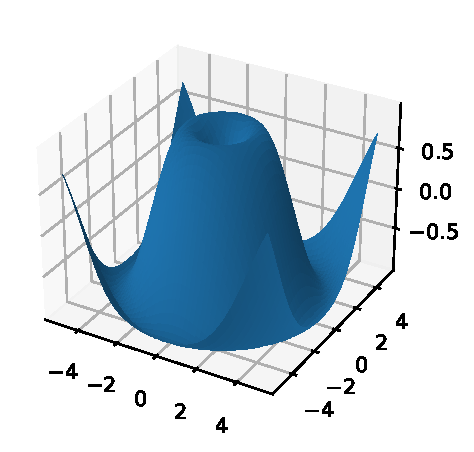
\includegraphics{index_files/figure-pdf/cell-2-output-1.pdf}

}

\end{figure}

\hypertarget{gruxe1fico-de-dispersiuxf3n}{%
\subsubsection{Gráfico de
dispersión}\label{gruxe1fico-de-dispersiuxf3n}}

Un gráfico de dispersión en 3D nos permite visualizar cómo los puntos se
distribuyen en un espacio tridimensional. A continuación, un ejemplo de
cómo crear un gráfico de dispersión utilizando Plotly:

\begin{Shaded}
\begin{Highlighting}[]
\ImportTok{import}\NormalTok{ plotly.graph\_objects }\ImportTok{as}\NormalTok{ go}

\CommentTok{\# Crear datos de ejemplo}
\NormalTok{x }\OperatorTok{=}\NormalTok{ [}\DecValTok{1}\NormalTok{, }\DecValTok{2}\NormalTok{, }\DecValTok{3}\NormalTok{, }\DecValTok{4}\NormalTok{, }\DecValTok{5}\NormalTok{]}
\NormalTok{y }\OperatorTok{=}\NormalTok{ [}\DecValTok{2}\NormalTok{, }\DecValTok{4}\NormalTok{, }\DecValTok{1}\NormalTok{, }\DecValTok{5}\NormalTok{, }\DecValTok{3}\NormalTok{]}
\NormalTok{z }\OperatorTok{=}\NormalTok{ [}\DecValTok{3}\NormalTok{, }\DecValTok{1}\NormalTok{, }\DecValTok{2}\NormalTok{, }\DecValTok{4}\NormalTok{, }\DecValTok{5}\NormalTok{]}

\CommentTok{\# Crear gráfico de dispersión}
\NormalTok{fig }\OperatorTok{=}\NormalTok{ go.Figure(data}\OperatorTok{=}\NormalTok{go.Scatter3d(x}\OperatorTok{=}\NormalTok{x, y}\OperatorTok{=}\NormalTok{y, z}\OperatorTok{=}\NormalTok{z, mode}\OperatorTok{=}\StringTok{\textquotesingle{}markers\textquotesingle{}}\NormalTok{))}

\CommentTok{\# Mostrar el gráfico}
\NormalTok{fig.show()}
\end{Highlighting}
\end{Shaded}

\begin{verbatim}
Unable to display output for mime type(s): text/html
\end{verbatim}

\begin{verbatim}
Unable to display output for mime type(s): text/html
\end{verbatim}

\hypertarget{gruxe1fico-de-contorno}{%
\subsubsection{Gráfico de contorno}\label{gruxe1fico-de-contorno}}

Un gráfico de contorno en 3D representa la variación de una variable en
un espacio tridimensional mediante líneas de contorno. Veamos un ejemplo
de cómo crear un gráfico de contorno utilizando Matplotlib:

\begin{Shaded}
\begin{Highlighting}[]
\ImportTok{import}\NormalTok{ numpy }\ImportTok{as}\NormalTok{ np}
\ImportTok{import}\NormalTok{ matplotlib.pyplot }\ImportTok{as}\NormalTok{ plt}

\CommentTok{\# Crear datos de ejemplo}
\NormalTok{x }\OperatorTok{=}\NormalTok{ np.linspace(}\OperatorTok{{-}}\DecValTok{5}\NormalTok{, }\DecValTok{5}\NormalTok{, }\DecValTok{100}\NormalTok{)}
\NormalTok{y }\OperatorTok{=}\NormalTok{ np.linspace(}\OperatorTok{{-}}\DecValTok{5}\NormalTok{, }\DecValTok{5}\NormalTok{, }\DecValTok{100}\NormalTok{)}
\NormalTok{X, Y }\OperatorTok{=}\NormalTok{ np.meshgrid(x, y)}
\NormalTok{Z }\OperatorTok{=}\NormalTok{ np.sin(np.sqrt(X}\OperatorTok{**}\DecValTok{2} \OperatorTok{+}\NormalTok{ Y}\OperatorTok{**}\DecValTok{2}\NormalTok{))}

\CommentTok{\# Crear gráfico de contorno}
\NormalTok{fig }\OperatorTok{=}\NormalTok{ plt.figure()}
\NormalTok{ax }\OperatorTok{=}\NormalTok{ fig.add\_subplot(}\DecValTok{111}\NormalTok{, projection}\OperatorTok{=}\StringTok{\textquotesingle{}3d\textquotesingle{}}\NormalTok{)}
\NormalTok{ax.contour3D(X, Y, Z)}

\CommentTok{\# Mostrar el gráfico}
\NormalTok{plt.show()}
\end{Highlighting}
\end{Shaded}

\begin{figure}[H]

{\centering 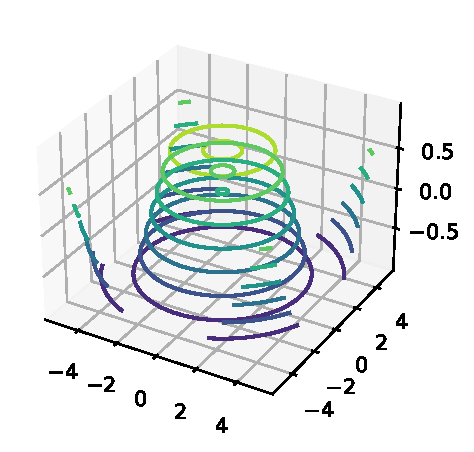
\includegraphics{index_files/figure-pdf/cell-4-output-1.pdf}

}

\end{figure}

Los gráficos de contorno son una forma efectiva de visualizar datos
tridimensionales en un formato bidimensional. Estos gráficos utilizan
líneas de contorno para representar las diferentes regiones de valores
en un plano.

En Python, puedes crear gráficos de contorno utilizando la función
\texttt{plt.contour()} de Matplotlib. Esta función toma los datos en
forma de matrices 2D y genera el gráfico de contorno correspondiente.

\begin{Shaded}
\begin{Highlighting}[]
\ImportTok{import}\NormalTok{ plotly.express }\ImportTok{as}\NormalTok{ px}
\ImportTok{import}\NormalTok{ pandas }\ImportTok{as}\NormalTok{ pd}
\ImportTok{import}\NormalTok{ folium}
\ImportTok{import}\NormalTok{ matplotlib.pyplot }\ImportTok{as}\NormalTok{ plt}
\ImportTok{import}\NormalTok{ numpy }\ImportTok{as}\NormalTok{ np}

\CommentTok{\# Datos de ejemplo}
\NormalTok{x }\OperatorTok{=}\NormalTok{ np.linspace(}\OperatorTok{{-}}\DecValTok{2}\NormalTok{, }\DecValTok{2}\NormalTok{, }\DecValTok{100}\NormalTok{)}
\NormalTok{y }\OperatorTok{=}\NormalTok{ np.linspace(}\OperatorTok{{-}}\DecValTok{2}\NormalTok{, }\DecValTok{2}\NormalTok{, }\DecValTok{100}\NormalTok{)}
\NormalTok{X, Y }\OperatorTok{=}\NormalTok{ np.meshgrid(x, y)}
\NormalTok{Z }\OperatorTok{=}\NormalTok{ np.sin(X}\OperatorTok{**}\DecValTok{2} \OperatorTok{+}\NormalTok{ Y}\OperatorTok{**}\DecValTok{2}\NormalTok{)}

\CommentTok{\# Crear gráfico de contorno}
\NormalTok{plt.contour(X, Y, Z)}

\CommentTok{\# Personalizar el gráfico}
\NormalTok{plt.title(}\StringTok{\textquotesingle{}Gráfico de contorno\textquotesingle{}}\NormalTok{)}
\NormalTok{plt.xlabel(}\StringTok{\textquotesingle{}Eje X\textquotesingle{}}\NormalTok{)}
\NormalTok{plt.ylabel(}\StringTok{\textquotesingle{}Eje Y\textquotesingle{}}\NormalTok{)}

\CommentTok{\# Mostrar el gráfico}
\NormalTok{plt.show()}
\end{Highlighting}
\end{Shaded}

\begin{figure}[H]

{\centering 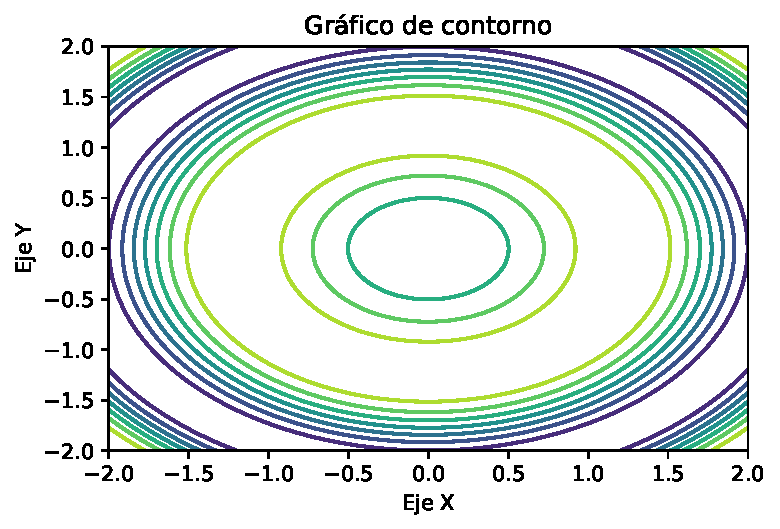
\includegraphics{index_files/figure-pdf/cell-5-output-1.pdf}

}

\end{figure}

En el código anterior, creamos una matriz 2D de valores \texttt{Z}
basados en los valores de las matrices \texttt{X} e \texttt{Y}. Luego
utilizamos \texttt{plt.contour()} para trazar el gráfico de contorno.
Puedes ajustar la apariencia del gráfico personalizando los títulos de
los ejes y agregando etiquetas.

Los gráficos de contorno son útiles para visualizar relaciones y
patrones en datos tridimensionales de manera más comprensible. Puedes
experimentar con diferentes configuraciones y colores para resaltar
áreas específicas o ajustar los niveles de contorno para obtener más
detalles.

\hypertarget{gruxe1ficos-3d-1}{%
\subsubsection{Gráficos 3D}\label{gruxe1ficos-3d-1}}

Los gráficos 3D son una forma visualmente impactante de representar
datos en tres dimensiones. Estos gráficos nos permiten explorar
relaciones complejas y patrones en nuestros datos de una manera más
inmersiva.

En Python, podemos crear gráficos 3D utilizando la biblioteca
Matplotlib. La función \texttt{plt.plot\_surface()} nos permite trazar
superficies 3D a partir de matrices de datos.

\begin{Shaded}
\begin{Highlighting}[]
\CommentTok{\# Datos de ejemplo}
\NormalTok{x }\OperatorTok{=}\NormalTok{ np.linspace(}\OperatorTok{{-}}\DecValTok{5}\NormalTok{, }\DecValTok{5}\NormalTok{, }\DecValTok{100}\NormalTok{)}
\NormalTok{y }\OperatorTok{=}\NormalTok{ np.linspace(}\OperatorTok{{-}}\DecValTok{5}\NormalTok{, }\DecValTok{5}\NormalTok{, }\DecValTok{100}\NormalTok{)}
\NormalTok{X, Y }\OperatorTok{=}\NormalTok{ np.meshgrid(x, y)}
\NormalTok{Z }\OperatorTok{=}\NormalTok{ np.sin(np.sqrt(X}\OperatorTok{**}\DecValTok{2} \OperatorTok{+}\NormalTok{ Y}\OperatorTok{**}\DecValTok{2}\NormalTok{))}

\CommentTok{\# Crear gráfico 3D}
\NormalTok{fig }\OperatorTok{=}\NormalTok{ plt.figure()}
\NormalTok{ax }\OperatorTok{=}\NormalTok{ fig.add\_subplot(}\DecValTok{111}\NormalTok{, projection}\OperatorTok{=}\StringTok{\textquotesingle{}3d\textquotesingle{}}\NormalTok{)}
\NormalTok{ax.plot\_surface(X, Y, Z)}

\CommentTok{\# Personalizar el gráfico}
\NormalTok{ax.set\_title(}\StringTok{\textquotesingle{}Gráfico 3D\textquotesingle{}}\NormalTok{)}
\NormalTok{ax.set\_xlabel(}\StringTok{\textquotesingle{}Eje X\textquotesingle{}}\NormalTok{)}
\NormalTok{ax.set\_ylabel(}\StringTok{\textquotesingle{}Eje Y\textquotesingle{}}\NormalTok{)}
\NormalTok{ax.set\_zlabel(}\StringTok{\textquotesingle{}Eje Z\textquotesingle{}}\NormalTok{)}

\CommentTok{\# Mostrar el gráfico}
\NormalTok{plt.show()}
\end{Highlighting}
\end{Shaded}

\begin{figure}[H]

{\centering 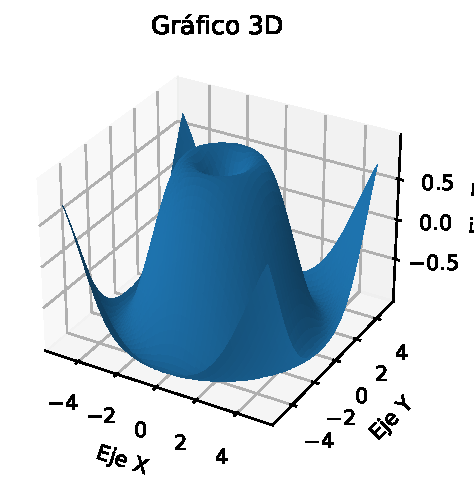
\includegraphics{index_files/figure-pdf/cell-6-output-1.pdf}

}

\end{figure}

En el código anterior, creamos matrices \texttt{X}, \texttt{Y} y
\texttt{Z} que representan los puntos de la superficie tridimensional.
Luego, utilizamos \texttt{plt.plot\_surface()} junto con la proyección
\texttt{\textquotesingle{}3d\textquotesingle{}} para trazar la
superficie en el gráfico 3D.

Puedes personalizar el gráfico ajustando los títulos de los ejes y
agregando etiquetas según sea necesario. Además, puedes experimentar con
diferentes configuraciones, como cambiar los colores, ajustar la
iluminación o agregar puntos de datos adicionales.

Los gráficos 3D son especialmente útiles cuando trabajamos con datos que
involucran múltiples variables. Nos permiten visualizar relaciones
complejas y descubrir patrones que podrían no ser evidentes en gráficos
bidimensionales.

Estos ejemplos te brindan una idea de cómo puedes utilizar gráficos de
superficie, dispersión y contorno en 3D para visualizar tus datos en un
espacio tridimensional. Experimenta con diferentes conjuntos de datos y
opciones de personalización para obtener visualizaciones impactantes y
comprensibles.

\hypertarget{gruxe1ficos-interactivos}{%
\section{Gráficos interactivos}\label{gruxe1ficos-interactivos}}

\hypertarget{utilizaciuxf3n-de-bibliotecas-como-plotly-y-bokeh-para-crear-gruxe1ficos-interactivos}{%
\subsection{Utilización de bibliotecas como Plotly y Bokeh para crear
gráficos
interactivos}\label{utilizaciuxf3n-de-bibliotecas-como-plotly-y-bokeh-para-crear-gruxe1ficos-interactivos}}

La visualización de datos se vuelve aún más emocionante cuando podemos
interactuar con los gráficos. Para lograr esto, podemos utilizar
bibliotecas como Plotly y Bokeh, que ofrecen poderosas herramientas para
crear gráficos interactivos. Veamos cómo utilizar estas bibliotecas:

\hypertarget{gruxe1ficos-interactivos-con-plotly}{%
\subsubsection{Gráficos interactivos con
Plotly}\label{gruxe1ficos-interactivos-con-plotly}}

Plotly es una biblioteca de visualización de datos que nos permite crear
gráficos interactivos con facilidad. A través de su interfaz intuitiva,
podemos explorar y analizar nuestros datos de manera dinámica. Aquí hay
un ejemplo de cómo crear un gráfico de dispersión interactivo con
Plotly:

\begin{Shaded}
\begin{Highlighting}[]
\ImportTok{import}\NormalTok{ plotly.express }\ImportTok{as}\NormalTok{ px}

\CommentTok{\# Cargar datos de ejemplo}
\NormalTok{data }\OperatorTok{=}\NormalTok{ px.data.iris()}

\CommentTok{\# Crear gráfico de dispersión interactivo}
\NormalTok{fig }\OperatorTok{=}\NormalTok{ px.scatter(data, x}\OperatorTok{=}\StringTok{"sepal\_width"}\NormalTok{, y}\OperatorTok{=}\StringTok{"sepal\_length"}\NormalTok{, color}\OperatorTok{=}\StringTok{"species"}\NormalTok{, hover\_data}\OperatorTok{=}\NormalTok{[}\StringTok{"petal\_length"}\NormalTok{, }\StringTok{"petal\_width"}\NormalTok{])}

\CommentTok{\# Mostrar el gráfico interactivo}
\NormalTok{fig.show()}
\end{Highlighting}
\end{Shaded}

\begin{verbatim}
Unable to display output for mime type(s): text/html
\end{verbatim}

Con Plotly, podemos personalizar nuestro gráfico, agregar colores y
etiquetas, y explorar los detalles de cada punto al pasar el cursor
sobre ellos.

\hypertarget{gruxe1ficos-interactivos-con-bokeh}{%
\subsubsection{Gráficos interactivos con
Bokeh}\label{gruxe1ficos-interactivos-con-bokeh}}

Bokeh es otra biblioteca popular que nos permite crear gráficos
interactivos en Python. Podemos utilizar Bokeh para crear
visualizaciones atractivas con herramientas de interacción, como zoom,
panorámica y selección. Aquí tienes un ejemplo de cómo crear un gráfico
de líneas interactivo con Bokeh:

\begin{Shaded}
\begin{Highlighting}[]
\CommentTok{\#pip install bokeh}

\ImportTok{from}\NormalTok{ bokeh.plotting }\ImportTok{import}\NormalTok{ figure, show}
\ImportTok{from}\NormalTok{ bokeh.io }\ImportTok{import}\NormalTok{ output\_notebook}

\CommentTok{\# Configurar la salida para mostrar en el notebook}
\NormalTok{output\_notebook()}

\CommentTok{\# Crear datos de ejemplo}
\NormalTok{x }\OperatorTok{=}\NormalTok{ [}\DecValTok{1}\NormalTok{, }\DecValTok{2}\NormalTok{, }\DecValTok{3}\NormalTok{, }\DecValTok{4}\NormalTok{, }\DecValTok{5}\NormalTok{]}
\NormalTok{y }\OperatorTok{=}\NormalTok{ [}\DecValTok{2}\NormalTok{, }\DecValTok{4}\NormalTok{, }\DecValTok{1}\NormalTok{, }\DecValTok{5}\NormalTok{, }\DecValTok{3}\NormalTok{]}

\CommentTok{\# Crear gráfico de líneas interactivo}
\NormalTok{p }\OperatorTok{=}\NormalTok{ figure(title}\OperatorTok{=}\StringTok{"Gráfico interactivo de líneas"}\NormalTok{, x\_axis\_label}\OperatorTok{=}\StringTok{"X"}\NormalTok{, y\_axis\_label}\OperatorTok{=}\StringTok{"Y"}\NormalTok{)}
\NormalTok{p.line(x, y)}

\CommentTok{\# Mostrar el gráfico interactivo}
\NormalTok{show(p)}
\end{Highlighting}
\end{Shaded}

\begin{verbatim}
Unable to display output for mime type(s): text/html
\end{verbatim}

\begin{verbatim}
Unable to display output for mime type(s): application/javascript, application/vnd.bokehjs_load.v0+json
\end{verbatim}

\begin{verbatim}
Unable to display output for mime type(s): text/html
\end{verbatim}

\begin{verbatim}
Unable to display output for mime type(s): application/javascript, application/vnd.bokehjs_exec.v0+json
\end{verbatim}

Con Bokeh, podemos explorar el gráfico de líneas interactivo utilizando
herramientas como el zoom y la panorámica. Además, podemos agregar
anotaciones y personalizar el diseño según nuestras necesidades.

Tanto Plotly como Bokeh nos ofrecen opciones versátiles para crear
gráficos interactivos, lo que nos permite comunicar nuestros datos de
manera más efectiva y atractiva. ¡Diviértete experimentando con estas
bibliotecas y lleva tus visualizaciones al siguiente nivel!

\hypertarget{ejemplos-pruxe1cticos-de-gruxe1ficos-interactivos-con-zoom-selecciuxf3n-y-herramientas-interactivas}{%
\subsection{Ejemplos prácticos de gráficos interactivos con zoom,
selección y herramientas
interactivas}\label{ejemplos-pruxe1cticos-de-gruxe1ficos-interactivos-con-zoom-selecciuxf3n-y-herramientas-interactivas}}

Ahora, vamos a explorar algunos ejemplos prácticos de gráficos
interactivos que utilizan funciones de zoom, selección y otras
herramientas interactivas. Estas características nos permiten explorar
los datos de manera más detallada y realizar análisis más profundos.
Veamos dos ejemplos utilizando las bibliotecas Plotly y Bokeh:

\hypertarget{ejemplo-1-gruxe1fico-interactivo-de-dispersiuxf3n-con-selecciuxf3n}{%
\subsubsection{Ejemplo 1: Gráfico interactivo de dispersión con
selección}\label{ejemplo-1-gruxe1fico-interactivo-de-dispersiuxf3n-con-selecciuxf3n}}

En este ejemplo, utilizaremos Plotly para crear un gráfico de dispersión
interactivo que nos permita seleccionar puntos específicos. Esto puede
ser útil cuando queremos resaltar ciertos puntos de interés en nuestros
datos. Aquí está el código:

\begin{Shaded}
\begin{Highlighting}[]
\CommentTok{\#pip install {-}{-}upgrade plotly}
\CommentTok{\#pip install dash}
\ImportTok{import}\NormalTok{ dash}
\ImportTok{import}\NormalTok{ dash\_core\_components }\ImportTok{as}\NormalTok{ dcc}
\ImportTok{import}\NormalTok{ dash\_html\_components }\ImportTok{as}\NormalTok{ html}
\ImportTok{import}\NormalTok{ plotly.express }\ImportTok{as}\NormalTok{ px}

\CommentTok{\# Cargar datos de ejemplo}
\NormalTok{data }\OperatorTok{=}\NormalTok{ px.data.iris()}

\CommentTok{\# Crear la aplicación Dash}
\NormalTok{app }\OperatorTok{=}\NormalTok{ dash.Dash(}\VariableTok{\_\_name\_\_}\NormalTok{)}

\CommentTok{\# Definir el diseño de la aplicación}
\NormalTok{app.layout }\OperatorTok{=}\NormalTok{ html.Div([}
\NormalTok{    dcc.Graph(}
        \BuiltInTok{id}\OperatorTok{=}\StringTok{\textquotesingle{}scatter{-}plot\textquotesingle{}}\NormalTok{,}
\NormalTok{        figure}\OperatorTok{=}\NormalTok{px.scatter(}
\NormalTok{            data, x}\OperatorTok{=}\StringTok{"sepal\_width"}\NormalTok{, y}\OperatorTok{=}\StringTok{"sepal\_length"}\NormalTok{, color}\OperatorTok{=}\StringTok{"species"}\NormalTok{,}
\NormalTok{            hover\_data}\OperatorTok{=}\NormalTok{[}\StringTok{"petal\_length"}\NormalTok{, }\StringTok{"petal\_width"}\NormalTok{]}
\NormalTok{        )}
\NormalTok{    )}
\NormalTok{])}

\CommentTok{\# Ejecutar la aplicación}
\ControlFlowTok{if} \VariableTok{\_\_name\_\_} \OperatorTok{==} \StringTok{\textquotesingle{}\_\_main\_\_\textquotesingle{}}\NormalTok{:}
\NormalTok{    app.run\_server(debug}\OperatorTok{=}\VariableTok{True}\NormalTok{)}
\end{Highlighting}
\end{Shaded}

\begin{verbatim}
<IPython.lib.display.IFrame at 0x7f6c3405fa30>
\end{verbatim}

Al seleccionar puntos en el gráfico, podemos obtener información
detallada sobre ellos y realizar análisis adicionales.

\hypertarget{ejemplo-2-gruxe1fico-interactivo-de-luxedneas-con-zoom-y-herramientas-interactivas}{%
\subsubsection{Ejemplo 2: Gráfico interactivo de líneas con zoom y
herramientas
interactivas}\label{ejemplo-2-gruxe1fico-interactivo-de-luxedneas-con-zoom-y-herramientas-interactivas}}

En este ejemplo, utilizaremos Bokeh para crear un gráfico de líneas
interactivo que nos permita hacer zoom y utilizar herramientas
interactivas adicionales. Esto es especialmente útil cuando tenemos
conjuntos de datos grandes y queremos explorar diferentes partes del
gráfico en detalle. Aquí tienes el código:

\begin{Shaded}
\begin{Highlighting}[]
\ImportTok{from}\NormalTok{ bokeh.plotting }\ImportTok{import}\NormalTok{ figure, show}
\ImportTok{from}\NormalTok{ bokeh.io }\ImportTok{import}\NormalTok{ output\_notebook}
\ImportTok{from}\NormalTok{ bokeh.models }\ImportTok{import}\NormalTok{ WheelZoomTool, HoverTool}

\CommentTok{\# Configurar la salida para mostrar en el notebook}
\NormalTok{output\_notebook()}

\CommentTok{\# Crear datos de ejemplo}
\NormalTok{x }\OperatorTok{=}\NormalTok{ [}\DecValTok{1}\NormalTok{, }\DecValTok{2}\NormalTok{, }\DecValTok{3}\NormalTok{, }\DecValTok{4}\NormalTok{, }\DecValTok{5}\NormalTok{]}
\NormalTok{y }\OperatorTok{=}\NormalTok{ [}\DecValTok{2}\NormalTok{, }\DecValTok{4}\NormalTok{, }\DecValTok{1}\NormalTok{, }\DecValTok{5}\NormalTok{, }\DecValTok{3}\NormalTok{]}

\CommentTok{\# Crear gráfico de líneas interactivo con zoom y herramientas interactivas}
\NormalTok{p }\OperatorTok{=}\NormalTok{ figure(title}\OperatorTok{=}\StringTok{"Gráfico interactivo de líneas"}\NormalTok{, x\_axis\_label}\OperatorTok{=}\StringTok{"X"}\NormalTok{, y\_axis\_label}\OperatorTok{=}\StringTok{"Y"}\NormalTok{, tools}\OperatorTok{=}\NormalTok{[WheelZoomTool(), HoverTool()])}
\NormalTok{p.line(x, y)}

\CommentTok{\# Mostrar el gráfico interactivo}
\NormalTok{show(p)}
\end{Highlighting}
\end{Shaded}

\begin{verbatim}
Unable to display output for mime type(s): text/html
\end{verbatim}

\begin{verbatim}
Unable to display output for mime type(s): application/javascript, application/vnd.bokehjs_load.v0+json
\end{verbatim}

\begin{verbatim}
Unable to display output for mime type(s): text/html
\end{verbatim}

\begin{verbatim}
Unable to display output for mime type(s): application/javascript, application/vnd.bokehjs_exec.v0+json
\end{verbatim}

Con este gráfico interactivo, podemos hacer zoom en áreas específicas,
obtener información detallada al pasar el cursor sobre los puntos y
explorar diferentes partes del gráfico según nuestras necesidades.

\hypertarget{gruxe1ficos-interactivos-1}{%
\subsection{Gráficos interactivos}\label{gruxe1ficos-interactivos-1}}

Los gráficos interactivos son una forma fascinante de visualizar datos y
permitir a los usuarios explorar la información de manera dinámica.
Python nos ofrece varias bibliotecas poderosas para crear gráficos
interactivos, como Plotly, Bokeh y Altair.

Una de las bibliotecas más populares para gráficos interactivos es
Plotly. Esta biblioteca nos permite crear gráficos interactivos con
características como zoom, pan y herramientas para resaltar puntos de
datos específicos. Además, Plotly proporciona una interfaz sencilla para
personalizar y diseñar nuestros gráficos.

\begin{Shaded}
\begin{Highlighting}[]
\CommentTok{\# Definir los datos y exportamos a un .csv}
\NormalTok{datos }\OperatorTok{=}\NormalTok{ \{}
    \StringTok{\textquotesingle{}nombre\textquotesingle{}}\NormalTok{: [}\StringTok{\textquotesingle{}Juan\textquotesingle{}}\NormalTok{, }\StringTok{\textquotesingle{}María\textquotesingle{}}\NormalTok{, }\StringTok{\textquotesingle{}Carlos\textquotesingle{}}\NormalTok{, }\StringTok{\textquotesingle{}Laura\textquotesingle{}}\NormalTok{],}
    \StringTok{\textquotesingle{}edad\textquotesingle{}}\NormalTok{: [}\DecValTok{25}\NormalTok{, }\DecValTok{30}\NormalTok{, }\DecValTok{35}\NormalTok{, }\DecValTok{28}\NormalTok{],}
    \StringTok{\textquotesingle{}salario\textquotesingle{}}\NormalTok{: [}\DecValTok{50000}\NormalTok{, }\DecValTok{60000}\NormalTok{, }\DecValTok{70000}\NormalTok{, }\DecValTok{55000}\NormalTok{],}
    \StringTok{\textquotesingle{}departamento\textquotesingle{}}\NormalTok{: [}\StringTok{\textquotesingle{}Ventas\textquotesingle{}}\NormalTok{, }\StringTok{\textquotesingle{}Marketing\textquotesingle{}}\NormalTok{, }\StringTok{\textquotesingle{}Finanzas\textquotesingle{}}\NormalTok{, }\StringTok{\textquotesingle{}Recursos Humanos\textquotesingle{}}\NormalTok{]}
\NormalTok{\}}

\CommentTok{\# Crear un DataFrame con los datos}
\NormalTok{df }\OperatorTok{=}\NormalTok{ pd.DataFrame(datos)}

\CommentTok{\# Guardar el DataFrame en un archivo CSV}
\NormalTok{df.to\_csv(}\StringTok{\textquotesingle{}datos.csv\textquotesingle{}}\NormalTok{, index}\OperatorTok{=}\VariableTok{False}\NormalTok{)}
\end{Highlighting}
\end{Shaded}

\begin{Shaded}
\begin{Highlighting}[]
\NormalTok{df }\OperatorTok{=}\NormalTok{ pd.read\_csv(}\StringTok{\textquotesingle{}datos.csv\textquotesingle{}}\NormalTok{)}

\CommentTok{\# Crear un gráfico interactivo de dispersión}
\NormalTok{fig }\OperatorTok{=}\NormalTok{ px.scatter(df, x}\OperatorTok{=}\StringTok{"edad"}\NormalTok{, y}\OperatorTok{=}\StringTok{"salario"}\NormalTok{,}
\NormalTok{                 color}\OperatorTok{=}\StringTok{"departamento"}\NormalTok{, hover\_data}\OperatorTok{=}\NormalTok{[}\StringTok{"nombre"}\NormalTok{])}

\CommentTok{\# Personalizar el diseño y las herramientas interactivas}
\NormalTok{fig.update\_layout(}
\NormalTok{    title}\OperatorTok{=}\StringTok{"Relación entre edad, salario y departamento"}\NormalTok{,}
\NormalTok{    xaxis\_title}\OperatorTok{=}\StringTok{"Edad"}\NormalTok{,}
\NormalTok{    yaxis\_title}\OperatorTok{=}\StringTok{"Salario"}\NormalTok{,}
\NormalTok{    hovermode}\OperatorTok{=}\StringTok{"closest"}
\NormalTok{)}

\CommentTok{\# Mostrar el gráfico interactivo}
\NormalTok{fig.show()}
\end{Highlighting}
\end{Shaded}

\begin{verbatim}
Unable to display output for mime type(s): text/html
\end{verbatim}

En el código anterior, utilizamos la biblioteca Plotly Express para
crear un gráfico interactivo de dispersión. Especificamos las columnas
del DataFrame que deseamos visualizar y personalizamos el gráfico con
títulos, etiquetas y configuraciones de interacción.

Además de Plotly, Bokeh y Altair también son bibliotecas populares para
crear gráficos interactivos en Python. Bokeh nos permite crear
visualizaciones interactivas basadas en navegadores web, mientras que
Altair se centra en la creación de gráficos declarativos y basados en
gramáticas.

Los gráficos interactivos son ideales para explorar datos, ya que
permiten a los usuarios interactuar con los gráficos y profundizar en la
información. Pueden ser utilizados para resaltar puntos de datos,
mostrar detalles adicionales en herramientas emergentes o incluso para
filtrar y seleccionar subconjuntos de datos.

Estos ejemplos ilustran cómo podemos aprovechar las herramientas
interactivas de las bibliotecas Plotly y Bokeh para crear
visualizaciones atractivas y explorar nuestros datos de manera más
eficiente.

\hypertarget{mapas-temuxe1ticos}{%
\section{Mapas temáticos}\label{mapas-temuxe1ticos}}

\hypertarget{introducciuxf3n-a-la-visualizaciuxf3n-de-datos-geoespaciales}{%
\subsection{Introducción a la visualización de datos
geoespaciales}\label{introducciuxf3n-a-la-visualizaciuxf3n-de-datos-geoespaciales}}

En esta sección, exploraremos la visualización de datos geoespaciales y
cómo podemos utilizarla para comprender mejor la información relacionada
con ubicaciones geográficas. Los mapas temáticos nos permiten
representar datos en un contexto geográfico, lo que facilita la
identificación de patrones, tendencias y relaciones espaciales.

\hypertarget{uso-de-bibliotecas-como-geopandas-plotly-y-folium-para-crear-mapas-temuxe1ticos}{%
\subsection{Uso de bibliotecas como Geopandas, Plotly y Folium para
crear mapas
temáticos}\label{uso-de-bibliotecas-como-geopandas-plotly-y-folium-para-crear-mapas-temuxe1ticos}}

Utilizaremos bibliotecas populares como Geopandas, Plotly y Folium para
crear mapas temáticos interactivos y personalizados. Estas herramientas
nos permiten cargar datos geoespaciales, agregar capas temáticas y
aplicar estilos visuales para resaltar información relevante en nuestros
mapas.

\hypertarget{geopandas}{%
\subsubsection{Geopandas}\label{geopandas}}

Geopandas es una biblioteca de Python que proporciona una manera fácil y
eficiente de trabajar con datos geoespaciales. Combina las capacidades
de las bibliotecas Pandas y Shapely para manejar y analizar datos
espaciales. Geopandas permite cargar, manipular y visualizar datos
geoespaciales, como formas de países, líneas de carreteras o puntos de
interés. Además, ofrece funcionalidades para realizar operaciones
espaciales y análisis geoespacial.

Para instalar Geopandas, puedes utilizar el gestor de paquetes de
Python, pip. Ejecuta el siguiente comando en tu terminal o entorno de
Python:

\begin{verbatim}
pip install geopandas
\end{verbatim}

Además de Geopandas, esta biblioteca depende de otras bibliotecas como
Pandas, Numpy y Shapely. Asegúrate de tenerlas instaladas previamente.

\hypertarget{plotly}{%
\subsubsection{Plotly}\label{plotly}}

Plotly es una biblioteca de visualización de datos interactiva que
permite crear gráficos y visualizaciones de alta calidad. Es
especialmente conocida por su capacidad de generar gráficos
interactivos, incluyendo mapas temáticos. Plotly ofrece una amplia gama
de gráficos, desde gráficos de barras y dispersión hasta gráficos 3D y
mapas interactivos. Además, permite personalizar la apariencia de los
gráficos y agregar interactividad como zoom, selección y herramientas de
exploración.

Para instalar Plotly, también puedes utilizar el gestor de paquetes pip.
Ejecuta el siguiente comando:

\begin{verbatim}
pip install plotly
\end{verbatim}

Plotly requiere la instalación de una biblioteca adicional llamada
Plotly.js. Puedes instalarla ejecutando el siguiente comando:

\begin{verbatim}
pip install plotly-geo
\end{verbatim}

\hypertarget{folium}{%
\subsubsection{Folium}\label{folium}}

Folium es una biblioteca de Python que se basa en Leaflet.js, una
biblioteca de JavaScript para visualización de mapas interactivos.
Folium facilita la creación de mapas interactivos y la superposición de
datos en ellos. Permite cargar datos geoespaciales en diferentes
formatos, como GeoJSON y Shapefiles, y agregar capas temáticas, como
polígonos coloreados, marcadores o líneas. Folium también ofrece
herramientas para personalizar la apariencia de los mapas y agregar
interactividad, como información emergente y controles de visualización.

La instalación de Folium también se puede realizar a través de pip.
Ejecuta el siguiente comando:

\begin{verbatim}
pip install folium
\end{verbatim}

Folium utiliza Leaflet.js como dependencia, por lo que no requiere
instalaciones adicionales.

Estas tres bibliotecas son herramientas poderosas para trabajar con
datos geoespaciales y crear mapas temáticos interactivos en Python. Cada
una tiene sus propias fortalezas y características, por lo que puedes
elegir la que mejor se adapte a tus necesidades y preferencias.
¡Experimenta con ellas y descubre cómo pueden enriquecer tus
visualizaciones geoespaciales!

\hypertarget{ejemplos-pruxe1cticos-de-mapas-de-calor-mapas-de-coropletas-y-mapas-de-puntos}{%
\section{Ejemplos prácticos de mapas de calor, mapas de coropletas y
mapas de
puntos}\label{ejemplos-pruxe1cticos-de-mapas-de-calor-mapas-de-coropletas-y-mapas-de-puntos}}

Exploraremos ejemplos prácticos de diferentes tipos de mapas temáticos
utilizando bibliotecas como Geopandas, Plotly y Folium. Estas
herramientas nos permiten visualizar datos geoespaciales de manera
efectiva. Veamos algunos ejemplos:

\hypertarget{ejemplo-1-mapa-de-calor}{%
\subsection{Ejemplo 1: Mapa de calor}\label{ejemplo-1-mapa-de-calor}}

Utilizaremos la biblioteca Plotly para crear un mapa de calor que
muestre la intensidad de un fenómeno en diferentes ubicaciones
geográficas. Aquí está el código:

\begin{Shaded}
\begin{Highlighting}[]
\ImportTok{import}\NormalTok{ plotly.graph\_objects }\ImportTok{as}\NormalTok{ go}

\CommentTok{\# Crear datos de ejemplo}
\NormalTok{locations }\OperatorTok{=}\NormalTok{ [}\StringTok{\textquotesingle{}New York\textquotesingle{}}\NormalTok{, }\StringTok{\textquotesingle{}Los Angeles\textquotesingle{}}\NormalTok{, }\StringTok{\textquotesingle{}Chicago\textquotesingle{}}\NormalTok{, }\StringTok{\textquotesingle{}Houston\textquotesingle{}}\NormalTok{, }\StringTok{\textquotesingle{}Phoenix\textquotesingle{}}\NormalTok{]}
\NormalTok{intensity }\OperatorTok{=}\NormalTok{ [}\DecValTok{100}\NormalTok{, }\DecValTok{200}\NormalTok{, }\DecValTok{150}\NormalTok{, }\DecValTok{300}\NormalTok{, }\DecValTok{250}\NormalTok{]}

\CommentTok{\# Crear el mapa de calor}
\NormalTok{fig }\OperatorTok{=}\NormalTok{ go.Figure(data}\OperatorTok{=}\NormalTok{go.Choropleth(}
\NormalTok{    locations}\OperatorTok{=}\NormalTok{locations,}
\NormalTok{    z}\OperatorTok{=}\NormalTok{intensity,}
\NormalTok{    locationmode}\OperatorTok{=}\StringTok{\textquotesingle{}USA{-}states\textquotesingle{}}\NormalTok{,}
\NormalTok{    colorscale}\OperatorTok{=}\StringTok{\textquotesingle{}Reds\textquotesingle{}}\NormalTok{,}
\NormalTok{    colorbar\_title}\OperatorTok{=}\StringTok{\textquotesingle{}Intensidad\textquotesingle{}}\NormalTok{,}
\NormalTok{))}

\CommentTok{\# Configurar el diseño del mapa}
\NormalTok{fig.update\_layout(}
\NormalTok{    title}\OperatorTok{=}\StringTok{\textquotesingle{}Mapa de calor\textquotesingle{}}\NormalTok{,}
\NormalTok{    geo\_scope}\OperatorTok{=}\StringTok{\textquotesingle{}usa\textquotesingle{}}\NormalTok{,}
\NormalTok{)}

\CommentTok{\# Mostrar el mapa de calor}
\NormalTok{fig.show()}
\end{Highlighting}
\end{Shaded}

\begin{verbatim}
Unable to display output for mime type(s): text/html
\end{verbatim}

En este ejemplo, hemos creado un mapa de calor que muestra la intensidad
de un fenómeno en diferentes ubicaciones geográficas en Estados Unidos.
Los datos de ejemplo incluyen nombres de ciudades y una medida de
intensidad asociada a cada ciudad.

\hypertarget{ejemplo-2-mapa-de-coropletas}{%
\subsection{Ejemplo 2: Mapa de
coropletas}\label{ejemplo-2-mapa-de-coropletas}}

Utilizaremos la biblioteca Geopandas para crear un mapa de coropletas
que muestre la distribución de un indicador específico en diferentes
regiones geográficas. Aquí está el código:

\begin{Shaded}
\begin{Highlighting}[]
\ImportTok{import}\NormalTok{ geopandas }\ImportTok{as}\NormalTok{ gpd}
\ImportTok{import}\NormalTok{ matplotlib.pyplot }\ImportTok{as}\NormalTok{ plt}

\CommentTok{\# Cargar datos geoespaciales de ejemplo}
\NormalTok{world }\OperatorTok{=}\NormalTok{ gpd.read\_file(gpd.datasets.get\_path(}\StringTok{\textquotesingle{}naturalearth\_lowres\textquotesingle{}}\NormalTok{))}

\CommentTok{\# Crear mapa de coropletas}
\NormalTok{world.plot(column}\OperatorTok{=}\StringTok{\textquotesingle{}pop\_est\textquotesingle{}}\NormalTok{, cmap}\OperatorTok{=}\StringTok{\textquotesingle{}OrRd\textquotesingle{}}\NormalTok{, legend}\OperatorTok{=}\VariableTok{True}\NormalTok{)}

\CommentTok{\# Mostrar el mapa de coropletas}
\NormalTok{plt.show()}
\end{Highlighting}
\end{Shaded}

\begin{figure}[H]

{\centering 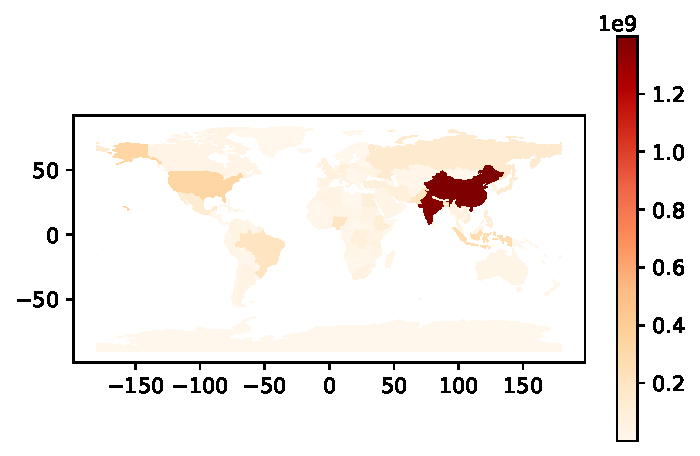
\includegraphics{index_files/figure-pdf/cell-14-output-1.pdf}

}

\end{figure}

Este mapa de coropletas nos permite visualizar la población estimada en
diferentes países o regiones.

\hypertarget{ejemplo-3-mapa-de-puntos}{%
\subsection{Ejemplo 3: Mapa de puntos}\label{ejemplo-3-mapa-de-puntos}}

Utilizaremos la biblioteca Folium para crear un mapa de puntos que
muestre la ubicación de puntos de interés en un área geográfica. Aquí
está el código:

\begin{Shaded}
\begin{Highlighting}[]
\ImportTok{import}\NormalTok{ folium}

\CommentTok{\# Crear mapa}
\NormalTok{mapa }\OperatorTok{=}\NormalTok{ folium.Map(location}\OperatorTok{=}\NormalTok{[}\FloatTok{51.5074}\NormalTok{, }\OperatorTok{{-}}\FloatTok{0.1278}\NormalTok{], zoom\_start}\OperatorTok{=}\DecValTok{12}\NormalTok{)}

\CommentTok{\# Agregar marcadores de puntos de interés}
\NormalTok{folium.Marker(location}\OperatorTok{=}\NormalTok{[}\FloatTok{51.5074}\NormalTok{, }\OperatorTok{{-}}\FloatTok{0.1278}\NormalTok{], popup}\OperatorTok{=}\StringTok{\textquotesingle{}Londres\textquotesingle{}}\NormalTok{).add\_to(mapa)}
\NormalTok{folium.Marker(location}\OperatorTok{=}\NormalTok{[}\FloatTok{48.8566}\NormalTok{, }\FloatTok{2.3522}\NormalTok{], popup}\OperatorTok{=}\StringTok{\textquotesingle{}París\textquotesingle{}}\NormalTok{).add\_to(mapa)}
\NormalTok{folium.Marker(location}\OperatorTok{=}\NormalTok{[}\FloatTok{40.7128}\NormalTok{, }\OperatorTok{{-}}\FloatTok{74.0060}\NormalTok{], popup}\OperatorTok{=}\StringTok{\textquotesingle{}Nueva York\textquotesingle{}}\NormalTok{).add\_to(mapa)}

\CommentTok{\# Mostrar el mapa de puntos}
\NormalTok{mapa}
\end{Highlighting}
\end{Shaded}

\begin{verbatim}
<folium.folium.Map at 0x7f6c30922dd0>
\end{verbatim}

Este mapa de puntos nos permite visualizar la ubicación de diferentes
ciudades en un área geográfica específica.

\hypertarget{gruxe1ficos-de-mapas}{%
\subsection{Gráficos de mapas}\label{gruxe1ficos-de-mapas}}

Los gráficos de mapas son una forma poderosa de visualizar datos
geoespaciales y resaltar patrones y distribuciones en un mapa
interactivo. Con Python, podemos utilizar diversas bibliotecas, como
Folium o Plotly, para crear gráficos de mapas personalizados.

Una de las bibliotecas más populares para gráficos de mapas es Folium.
Esta biblioteca nos permite crear mapas interactivos utilizando datos
geoespaciales y agregar capas adicionales, como marcadores o polígonos.

\begin{Shaded}
\begin{Highlighting}[]
\CommentTok{\# pip install folium}

\CommentTok{\# Crear un mapa}
\NormalTok{mapa }\OperatorTok{=}\NormalTok{ folium.Map(location}\OperatorTok{=}\NormalTok{[}\FloatTok{40.7128}\NormalTok{, }\OperatorTok{{-}}\FloatTok{74.0060}\NormalTok{], zoom\_start}\OperatorTok{=}\DecValTok{10}\NormalTok{)}

\CommentTok{\# Agregar un marcador}
\NormalTok{folium.Marker(location}\OperatorTok{=}\NormalTok{[}\FloatTok{40.7128}\NormalTok{, }\OperatorTok{{-}}\FloatTok{74.0060}\NormalTok{], popup}\OperatorTok{=}\StringTok{\textquotesingle{}Nueva York\textquotesingle{}}\NormalTok{).add\_to(mapa)}

\CommentTok{\# Mostrar el mapa}
\NormalTok{mapa}
\end{Highlighting}
\end{Shaded}

\begin{verbatim}
<folium.folium.Map at 0x7f6c30923250>
\end{verbatim}

En el código anterior, creamos un mapa centrado en una ubicación
específica (latitud y longitud) utilizando \texttt{folium.Map()}. Luego,
agregamos un marcador en la misma ubicación utilizando
\texttt{folium.Marker()}. Puedes personalizar el marcador y agregar
información adicional, como un mensaje emergente, para proporcionar más
detalles.

Folium también nos permite agregar capas adicionales, como polígonos o
rutas, utilizando funciones como \texttt{folium.Polygon()} o
\texttt{folium.PolyLine()}. Estas capas pueden ayudarnos a representar
datos geoespaciales más complejos y enriquecer nuestra visualización.

Otra biblioteca popular para gráficos de mapas es Plotly, que nos ofrece
capacidades de visualización interactiva y personalizable. Con Plotly,
podemos crear mapas con múltiples capas y utilizar técnicas de
visualización avanzadas, como el mapa de calor o la agregación espacial.

Los gráficos de mapas son especialmente útiles para visualizar datos
geoespaciales, como ubicaciones de tiendas, distribución de población o
rutas. Nos permiten comprender mejor la información cuando está
relacionada con la ubicación geográfica.

Estos ejemplos ilustran cómo podemos utilizar las bibliotecas Geopandas,
Plotly y Folium para crear mapas temáticos que resalten información
geoespacial de manera efectiva. ¡Diviértete explorando diferentes tipos
de mapas y descubre nuevas perspectivas en tus datos geoespaciales!

\hypertarget{casos-de-estudio-y-ejemplos-pruxe1cticos}{%
\section{Casos de estudio y ejemplos
prácticos}\label{casos-de-estudio-y-ejemplos-pruxe1cticos}}

\hypertarget{aplicaciuxf3n-de-gruxe1ficos-avanzados-en-escenarios-reales}{%
\subsection{Aplicación de gráficos avanzados en escenarios
reales}\label{aplicaciuxf3n-de-gruxe1ficos-avanzados-en-escenarios-reales}}

En el ámbito científico, los gráficos avanzados pueden ayudarnos a
representar datos experimentales, modelados matemáticos y resultados de
investigaciones. Podremos visualizar relaciones complejas, patrones y
tendencias en los datos, lo que nos permitirá obtener una comprensión
más profunda de los fenómenos estudiados.

En el mundo empresarial, los gráficos avanzados son una herramienta
poderosa para presentar datos financieros, análisis de mercado y
resultados de proyectos. Estos gráficos nos permiten identificar
oportunidades de crecimiento, evaluar el desempeño de productos o
servicios, y comunicar estrategias de manera clara y persuasiva.

En el campo de la geografía y la cartografía, los gráficos avanzados nos
ayudan a visualizar datos espaciales y crear mapas temáticos. Podremos
representar variables geográficas como densidad de población,
distribución de recursos naturales o patrones de movimiento, lo que nos
facilitará el análisis y la toma de decisiones en temas como urbanismo,
planificación territorial y conservación ambiental.

\hypertarget{ejemplos-de-visualizaciuxf3n-de-datos-en-campos-como-ciencia-negocios-geografuxeda-etc.}{%
\subsection{Ejemplos de visualización de datos en campos como ciencia,
negocios, geografía,
etc.}\label{ejemplos-de-visualizaciuxf3n-de-datos-en-campos-como-ciencia-negocios-geografuxeda-etc.}}

En el ámbito científico, podemos utilizar gráficos avanzados para
representar datos experimentales y resultados de investigaciones. Por
ejemplo, podemos crear gráficos de líneas para mostrar la evolución
temporal de variables en un experimento, o gráficos de dispersión para
analizar la relación entre dos variables. Estos gráficos nos ayudan a
identificar patrones, tendencias y correlaciones en los datos
científicos.

En el mundo empresarial, la visualización de datos es fundamental para
comprender el rendimiento de un negocio y tomar decisiones estratégicas.
Podemos utilizar gráficos avanzados para representar datos financieros,
como gráficos de barras para comparar ventas por categoría o gráficos de
torta para mostrar la participación de mercado de diferentes productos.
Estos gráficos nos permiten identificar oportunidades de mejora, evaluar
el éxito de nuestras estrategias y comunicar de manera efectiva a los
interesados.

En el campo de la geografía, los gráficos avanzados nos ayudan a
visualizar datos espaciales y crear mapas temáticos. Por ejemplo,
podemos utilizar gráficos de coropletas para representar la densidad de
población en diferentes regiones, o gráficos de puntos para mostrar la
ubicación de sitios de interés. Estos gráficos nos permiten comprender
mejor la distribución geográfica de los datos y tomar decisiones
informadas en temas como planificación urbana, gestión de recursos
naturales y desarrollo sostenible.

\hypertarget{anuxe1lisis-de-datos-complejos-utilizando-gruxe1ficos-avanzados}{%
\subsection{Análisis de datos complejos utilizando gráficos
avanzados}\label{anuxe1lisis-de-datos-complejos-utilizando-gruxe1ficos-avanzados}}

Un ejemplo común de análisis de datos complejos es el estudio de redes y
relaciones. Utilizando gráficos avanzados, podemos representar y
analizar redes sociales, redes de colaboración científica, interacciones
entre personas, entre otros. Los gráficos de redes nos ayudan a
identificar comunidades, detectar influencias y comprender la estructura
de las relaciones en un conjunto de datos.

Otro ejemplo es el análisis de datos multivariables, donde tenemos
múltiples variables que se relacionan entre sí. Utilizando gráficos
avanzados como los gráficos de dispersión en varias dimensiones, los
gráficos de radar o los gráficos de superficie, podemos visualizar y
explorar las relaciones complejas entre múltiples variables. Esto nos
permite identificar patrones, tendencias y correlaciones que podrían
pasar desapercibidos en un análisis univariable.

Además, los gráficos avanzados nos brindan herramientas interactivas que
nos permiten explorar los datos en detalle. Podemos aplicar filtros,
hacer zoom, obtener información detallada al pasar el cursor sobre los
elementos del gráfico y realizar comparaciones dinámicas. Esto facilita
el análisis exploratorio de datos y nos ayuda a descubrir información
oculta o insights inesperados.

\hypertarget{conclusiones-y-recursos-adicionales}{%
\section{Conclusiones y recursos
adicionales}\label{conclusiones-y-recursos-adicionales}}

En este blog, hemos explorado el fascinante mundo de los gráficos
avanzados con Python. Hemos aprendido cómo utilizar bibliotecas como
Matplotlib, Seaborn, Plotly, y Folium para crear visualizaciones
impactantes y efectivas.

Algunas de las conclusiones clave que hemos obtenido son:

\begin{itemize}
\tightlist
\item
  Los gráficos avanzados nos permiten representar datos complejos de
  manera clara y comprensible.
\item
  La elección adecuada de gráficos es fundamental para transmitir la
  información de manera efectiva.
\item
  Las bibliotecas de Python ofrecen una amplia variedad de herramientas
  y opciones para crear visualizaciones interactivas y atractivas.
\item
  La personalización y la atención a los detalles son importantes para
  lograr gráficos de alta calidad.
\end{itemize}

Para seguir aprendiendo sobre gráficos avanzados, te recomendamos los
siguientes recursos adicionales:

\begin{itemize}
\tightlist
\item
  Documentación oficial de las bibliotecas: Matplotlib, Seaborn, Plotly,
  Folium.
\item
  Tutoriales en línea y cursos especializados en visualización de datos
  con Python.
\item
  Blogs y libros sobre visualización de datos que aborden técnicas
  avanzadas y mejores prácticas.
\end{itemize}

¡Explora, experimenta y diviértete creando gráficos avanzados con
Python! Recuerda que la visualización de datos es una herramienta
poderosa para comunicar y analizar información de manera efectiva.

\hypertarget{publicaciones-similares}{%
\section{Publicaciones Similares}\label{publicaciones-similares}}

Si te interesó este artículo, te recomendamos que explores otros blogs y
recursos relacionados que pueden ampliar tus conocimientos. Aquí te dejo
algunas sugerencias:

\begin{enumerate}
\def\labelenumi{\arabic{enumi}.}
\item
  \href{../2023-06-22-01-introduccion-a-python/index.qmd}{Introducción}
\item
  \href{../2023-06-23-02-variables-expresiones-y-statements-con-python/index.qmd}{Variables,
  expresiones y statements}
\item
  \href{../2023-06-24-03-objetos-de-python/index.qmd}{Objetos de Python}
\item
  \href{../2023-06-25-04-ejecucion-condicional-con-python/index.qmd}{Ejecución
  condicional}
\item
  \href{../2023-06-26-05-iteraciones-con-python/index.qmd}{Iteraciones}
\item
  \href{../2023-06-27-06-funciones-con-python/index.qmd}{Funciones}
\item
  \href{../2023-06-28-07-dataframes-con-python/index.qmd}{Dataframes}
\item
  \href{../2023-06-29-introduccion-a-la-visualizacion-de-datos-con-python/index.qmd}{Introducción
  a la visualización de datos}
\item
  \href{../2023-06-30-graficos-avanzados-con-python/index.qmd}{Gráficos
  avanzados}
\item
  \href{../2023-07-01-visualizacion-de-datos-en-tiempo-real-con-python/index.qmd}{Visualización
  de datos en tiempo real}
\item
  \href{../2023-07-02-visualizacion-de-datos-en-finanzas-con-python/index.qmd}{Visualización
  de datos en finanzas}
\item
  \href{../2023-07-03-visualizacion-de-datos-en-microeconomia-con-python/index.qmd}{Visualización
  de datos en microeconomía}
\item
  \href{../2023-07-04-visualizacion-de-datos-en-macroeconomia-con-python/index.qmd}{Visualización
  de datos en macroeconomía}
\item
  \href{../2023-07-05-visualizacion-de-datos-en-estadistica-con-python/index.qmd}{Visualización
  de datos en estadística}
\item
  \href{../2023-07-06-visualizacion-de-datos-en-econometria-con-python/index.qmd}{Visualización
  de datos en econometría}
\item
  \href{../2023-07-07-mejores-practicas-y-consejos-de-visualizacion-de-datos-con-python/index.qmd}{Mejores
  prácticas y consejos de visualización de datos}
\item
  \href{../2023-07-08-08-prediccion-y-metrica-de-performance-con-python/index.qmd}{Predicción
  y métrica de performance}
\item
  \href{../2023-07-09-09-metodos-de-machine-learning-para-clasificacion-con-python/index.qmd}{Métodos
  de machine learning para clasificación}
\item
  \href{../2023-07-10-10-metodos-de-machine-learning-para-regresion-con-python/index.qmd}{Métodos
  de machine learning para regresión}
\item
  \href{../2023-07-11-11-validacion-cruzada-y-composicion-del-modelo-con-python/index.qmd}{Validación
  cruzada y composición del modelo}
\end{enumerate}

Esperamos que encuentres estas publicaciones igualmente interesantes y
útiles. ¡Disfruta de la lectura!


\printbibliography


\end{document}
